\section{Z80emu{\dywiz}gui}

Moduł \emph{Z80emu{\dywiz}gui} implementuje interfejs użytkownika zaprezentowany na rysunku nr \ref{img:z80Gui}. Został on napisany z pomocą biblioteki \emph{JavaFX}. Największą jej zaletą w porównaniu do poprzedniczki, którą była biblioteka \emph{Swing}, jest możliwość definiowania widoku aplikacji za pomocą języków XML i CSS. Projektowanie interfejsu w \emph{JavaFx} przypomina nieco tworzenie strony WWW.

Kod źródłowy implementujący interfejs użytkownika został podzielony na pakiety, których strukturę przedstawiono na rysunku \ref{img:z80EmuGuiPackage}. Postanowiono podzielić pliki zgodnie ze wzorcem \emph{Model-View-Controller}, który dzieli aplikacje na trzy główne części. Każda z~nich ma swoją reprezentację w module jako oddzielna paczka:
\begin{itemize}
    \item \emph{model} - implementuje logikę biznesową. W tym przypadku, między innymi zarządza procesem asemblacji i emulacji.
    \item \emph{View} - opisuje widok aplikacji. W projektach zbudowanych za pomocą \emph{javaFx} są to pliki XML i CSS. Oprócz nich mogą też być pliki języka Java, odpowiedzialne za prezentację danych. W opisywanym projekcie są to np. klasy, których zadaniem jest kolorowanie składni w edytorze kodu asemblera, tworzenie okien dialogowych lub system pomocy.
    \item \emph{controller} - zadaniem kontrolera jest przetworzenie informacji od użytkownika, by na jej podstawie wywoływać metody modelu i aktualizować widok. W projekcie każda część interfejsu posiada osobny kontroler (dla przykładu, osobne kontrolery zajmują się pamięcią programu, przerwaniami, i edytorem kodu asemblera).
\end{itemize}

\begin{figure}[h]
		\centering
		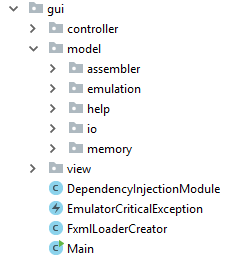
\includegraphics[width=0.4\textwidth]{z80EmuGuiPackage}
		\caption{Podział na pakiety modułu z80emu{\dywiz}gui}
		\label{img:z80EmuGuiPackage}
\end{figure}



\subsection{Wstrzykiwanie zależności za pomocą biblioteki \emph{Guice}}
Wstrzykiwanie zależności (z ang. \emph{Dependency Injection}) to technika programowania, której głównym założeniem jest przekazywanie gotowych skonfigurowanych już obiektów do innych (wstrzykiwanie ich), które ich wymagają. Moduł interfejsu użytkownika posiada wiele współpracujących ze sobą  klas. Zarządzanie nimi stało się z czasem uciążliwe. Problem postanowiono rozwiązać z pomocą biblioteki \emph{Guice}, która implementuje technikę wstrzykiwania zależności.

Aby opisać problem, należy przedstawić, z jakich elementów zostały zbudowane kontrolery w projekcie. Fragment jednego z nich został zaprezentowany w listingu \ref{listing:z80DiCOntrollerExample}. Kontroler ten jest zależny od modelu (linie nr 3-5) oraz posiada obiekty wstrzykiwane przez bibliotekę graficzną na podstawie plików FXML (linie nr 7 i 8). Zatem należało użyć biblioteki \emph{Guice} nie wprowadzając przy tym konfliktów z \emph{JavaFX}.

\begin{listing}[h]
	\inputminted{java}{listings/z80emu-gui/DiControllerExample.java}
	\caption{Zależności klasy \emph{MemoryController}}
	\label{listing:z80DiCOntrollerExample}
\end{listing}

Połączono \emph{JavaFx} i \emph{Guice} w następujący sposób. Interfejs biblioteki graficznej posiada metodę \emph{setControllerFactory(Callback<Class<?>, Object> controllerFactory)}, potrafiącą podmienić domyślną fabrykę kontrolerów. Jako jej parametr przekazano metodę biblioteki \emph{Guice} \emph{<T> T getInstance(Class<T> type)}, która zwraca instancję danego obiektu. Dzięki takiemu rozwiązaniu, kontrolery mają możliwość używania wszystkich adnotacji ułatwiających wstrzykiwanie do nich zależności (a nawet innych kontrolerów) i jednocześnie są udekorowane w~obiekty biblioteki graficznej.

\subsection{Integracja z projektem Z80emu{\dywiz}core}

\begin{listing}[h]
	\inputminted{java}{listings/z80emu-gui/EmulatorThread.java}
	\caption{Klasa \emph{EmulatorThread} realizująca emulację w trybie ciągłym}
	\label{listing:emulatorThread}
\end{listing}

\emph{Z80emu{\dywiz}gui} używa do emulacji modułu \emph{Z80emu{\dywiz}core}, który zawiera metodę \emph{runOneInstruction} wykonującą kolejną instrukcję CPU. Pomiędzy jej kolejnymi wywołaniami powinny zostać zgłoszone przerwania lub odczytane wartości rejestrów, pamięci i flag. Aby umożliwić to zarówno w trybie ciągłym, jak i krokowym wymagane było umieszczenie emulacji w osobnym wątku.

W tym celu wykonano klasę \emph{EmulatorThread}, którą pokazano w listingu \ref{listing:emulatorThread}. Użytkownik może uruchomić i zatrzymać emulację w dowolnym momencie za pomocą publicznych metod \emph{pause} i \emph{unPause}.

Metoda \emph{pause}, która docelowo zostaje wywoływana z innego wątku, zmienia wartość pola \emph{pause} typu \emph{boolean} na \emph{false}.  W głównej pętli emulacji sprawdzany jest warunek \emph{if(pause) \{lock.wait(); pause = false;\}}. Jeśli jest on spełniony, to wątek jest wprowadzany w stan oczekiwania.

Metoda \emph{unPause}, która także wywoływana jest z innego wątku, odblokowuje wątek, i~pozwala wznowić emulację.

% pomysły co mogło by się znaleźć w tym dziale: 
% - o wątkach, jak zaimplementowałem debugowanie ciągłe

% - podział na kontrolery, że jest wiele kontrolerów a nie jeden główny
% - opisać, jak podpiąłem biblioteke asemblującą, wspomnieć że to nie jest moje dzieło
% - ?? opisać jak działają przerwania
% - 
% - w jaki sposób zaimplementowano wiki, że jest to rekurencja itp. Wspomnieć że pliki jar nie mają struktury katalogów, i nie da się w nich wylistować listy plików w danym katalogu, dlatego tak to skomplikowałem
% - info co zostało niepodpięte pod gui, np przerwania

